\chapter{Further Strong-Interaction Results}\label{App:Strong_Interactions}

\section{Higher-Order Corrections to Doublon Energies}\label{App:DoublonHigherOrder}

This appendix presents details of the higher-order corrections to the effective doublon Hamiltonian. Fig. \ref{Fig:Doublon_Energy_Difference} shows the difference $\Delta E$ between the the effective single-particle energies calculated using Eq. \ref{Eq:DoublonHamiltonian}, and numerical doublon energies, $E_d$ (with the energy offset $E_0$ subtracted). $\Delta E$ is found to scale linearly with $E_d$. This explains the observed dynamical behaviour in Fig. \ref{Fig:Doublon_SingleSite_Evolution}, where the data for the doublons and the effective single particle appear identical up to a linear re-scaling of the time axis. 

Fig. \ref{Fig:Doublon_Energy_Difference_vs_U} demonstrates that $\Delta E$ arises due to next-highest-order hopping processes, giving energy corrections $\propto \frac{J^3}{U^2}$. The plot shows that the fitted linear gradient of $\Delta E$ with $E_d$ is $\appropto U^{-1}$. Since the gradient is $\propto \frac{\Delta E}{E_d}$, and $E_d\propto U^{-1}$ to leading order, this demonstrates that $\Delta E\propto U^{-2}$, as predicted.

This scaling of $\Delta E$ with $U$ does not explain why the relationship between $\Delta E$ and $E_d$ should be linear. Since the values involved are $\ll1$, it is possible that this linear behaviour is the leading order term of a more complicated relationship. Alternatively, there may be an underlying theoretical reason that the relationship is truly linear; the extremely high accuracy of the linear fit seems to support this. As this is only a minor detail in understanding the doublon behaviour, it was not investigated further.

\newpage

\begin{figure}[t!]
    \centering
    \sidesubfloat[]{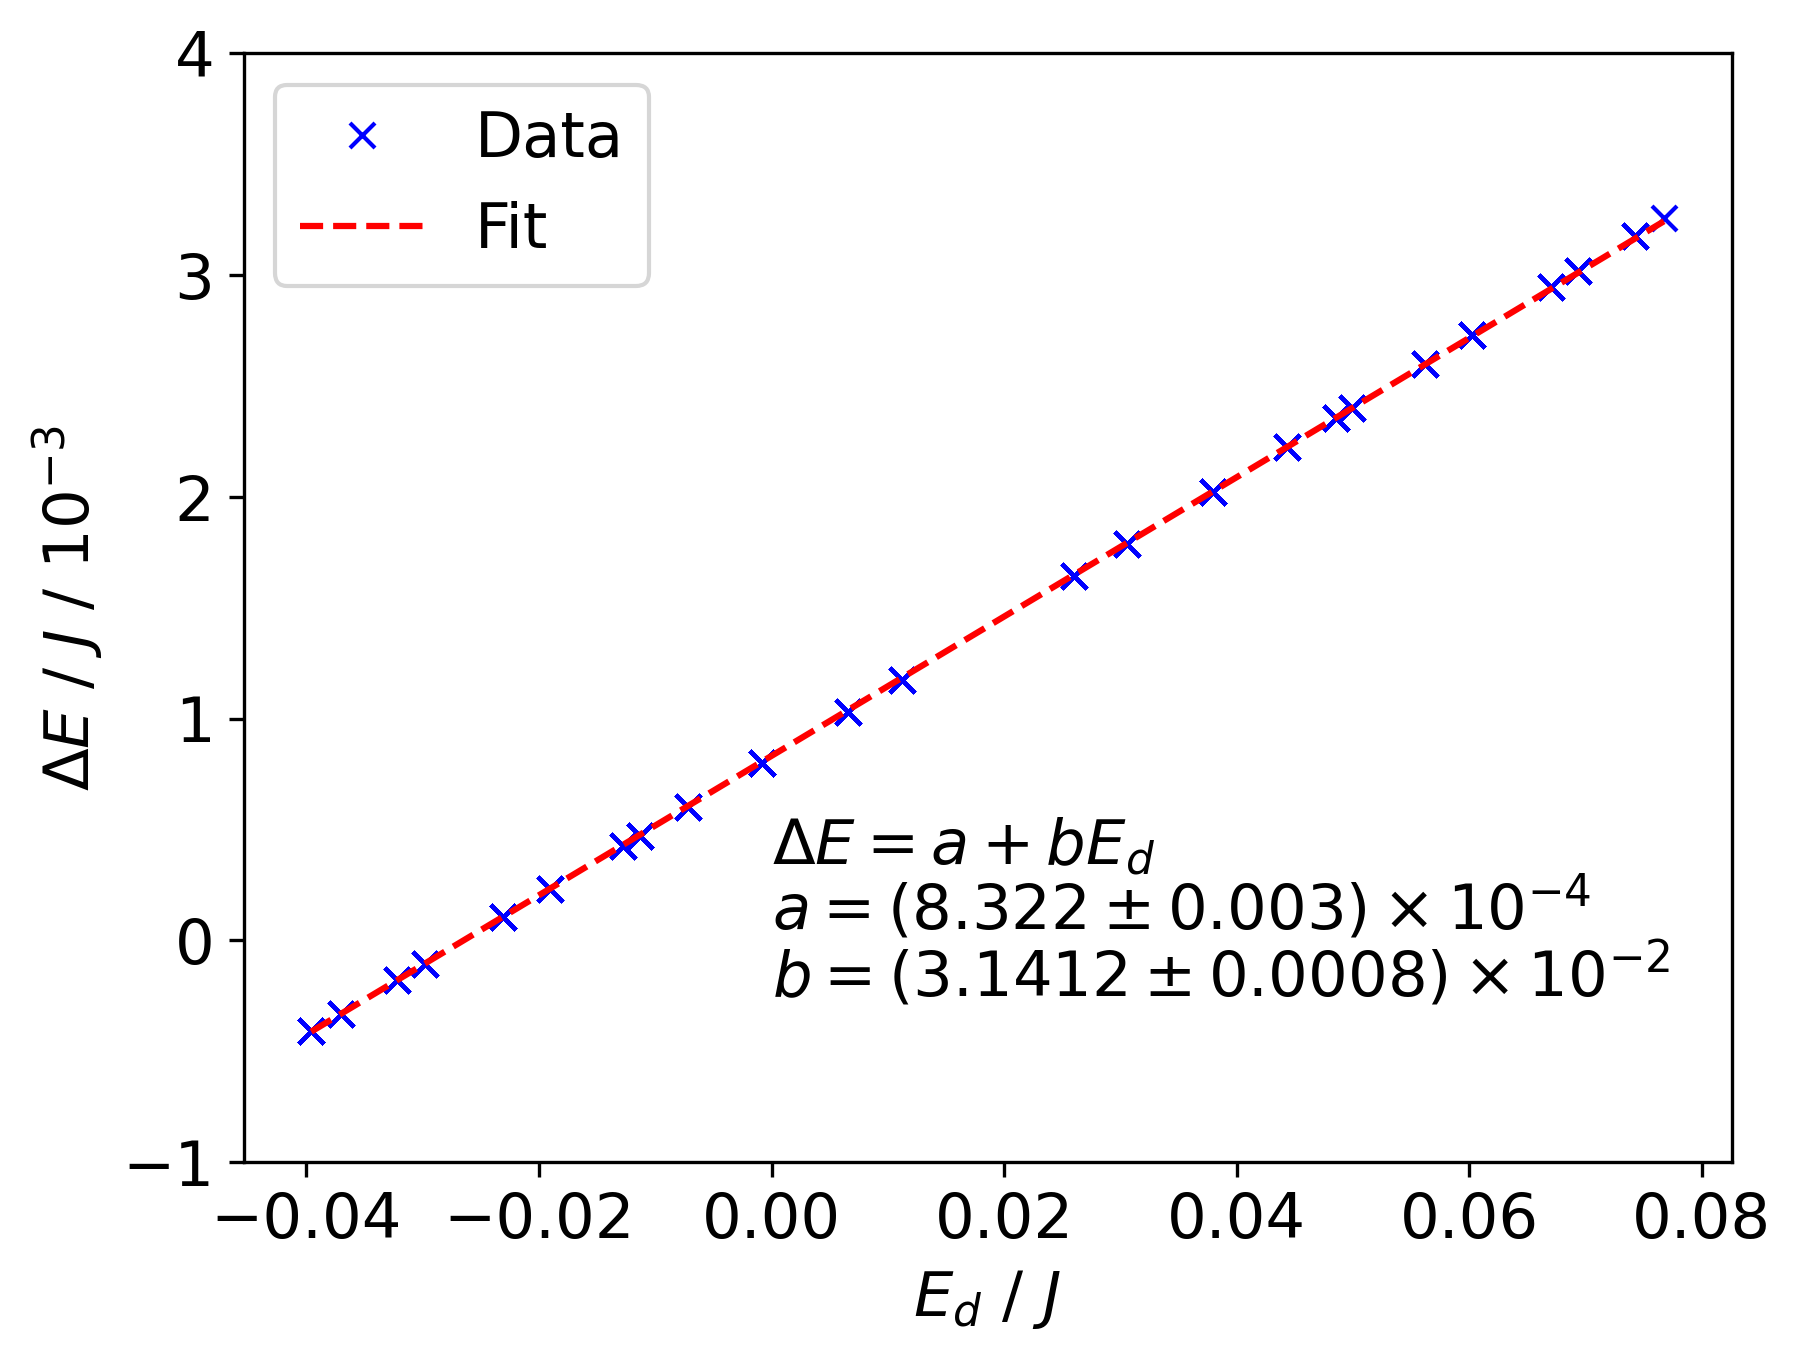
\includegraphics[height=5.6cm]{Figures/Doublon_Energy_Difference}\label{Fig:Doublon_Energy_Difference}}\hfill
    \sidesubfloat[]{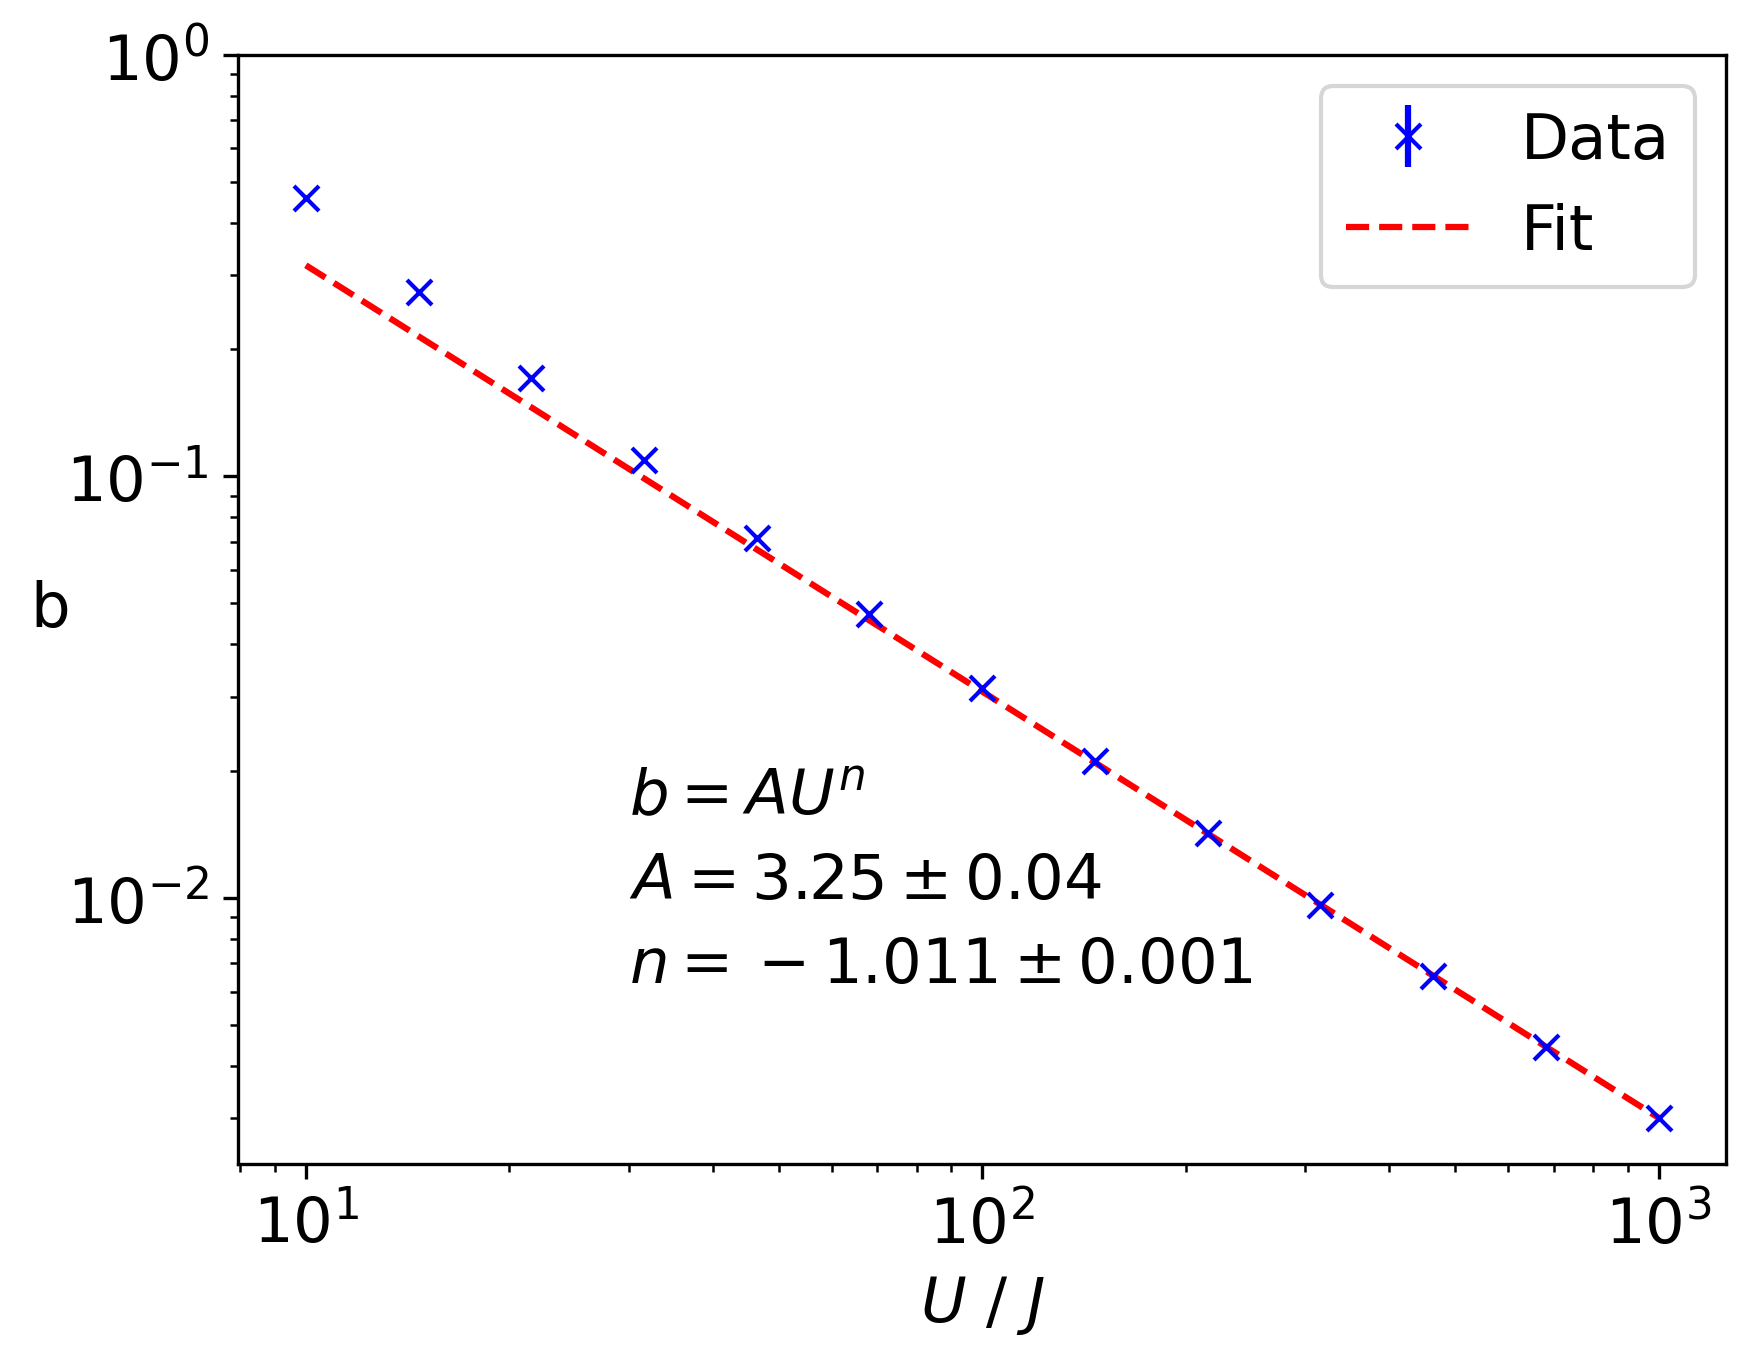
\includegraphics[height=5.6cm]{Figures/Doublon_Energy_Difference_vs_U}\label{Fig:Doublon_Energy_Difference_vs_U}}
    \caption{(a) Energy difference $\Delta E$ between numerical doublon energies, $E_d$, and effective single-particle energies (Eq. \ref{Eq:DoublonHamiltonian}), against $E_d$, for $U/J=100$. The energy offset $E_0$ is subtracted from $E_d$. A linear fit is performed to the data. (b) Values of the gradient, $b$, fitted to data of $\Delta E$ against $E_d$ (as depicted in (a)), for different $U$. The power law fit is performed to the data for $U\geq100$.}
    \label{Fig:Doublon_Higher_Order}
\end{figure}
\text{}

\section{Doublon Fraction}\label{App:Doublon_Fraction}

In this appendix, it is verified that for $U\gg J$, particles initially in a doublon state do not separate, but instead remain together as a composite particle. The doublon fraction, or probability that the two particles occupy a doublon state, at time $t$ is:
\begin{equation}
    P_{\text{d}}(t)=\sum_{i}|\langle d_i|\Psi(t)\rangle|^2
\end{equation}
The sum runs over lattice sites $i$. Fig. \ref{Fig:Pd_vs_t} shows $P_d(t)$ for simulations with two particles initially in a doublon state (on the same site), for various $U$. In all cases, there is an initial transient period, before a steady-state period of fluctuations around a constant mean value. The time-averaged steady-state $\overline{P_d}$ is plotted against $U$ in Fig. \ref{Fig:Pd_vs_U}. For $U/J\gg1$, this tends to 1; as expected, the particles cannot separate, and instead the doublon propagates through the lattice as a composite particle. Furthermore, in Fig. \ref{Fig:Pd_vs_U_log}, $1-\overline{P_d}$ decreases $\appropto U^{-2}$ for large $U$. This is consistent with a perturbation-theory admixture of scattering states, with amplitude $\propto U^{-1}$ and therefore probability $\propto U^{-2}$. For weak interactions, $\overline{P_d}\sim N_{\text{sites}}/N_{\text{states}}$, the value expected for no correlations; the particles equally occupy all $N_{\text{states}}$ basis states, of which $N_{\text{sites}}$ are doublon states. This value is slightly exceeded due to the large spikes in $P_d$ visible in Fig. \ref{Fig:Pd_vs_t}, which are due to degenerate eigenstates interfering in phase. As with the simulation of scattering states in Fig. \ref{Fig:Scattering_Evolution}, stronger interactions lift this degeneracy, suppressing the spikes.

\vspace{1cm}

%Don't really like this with the initial density figure
\begin{figure}[ht]
    \centering
    %\sidesubfloat[]{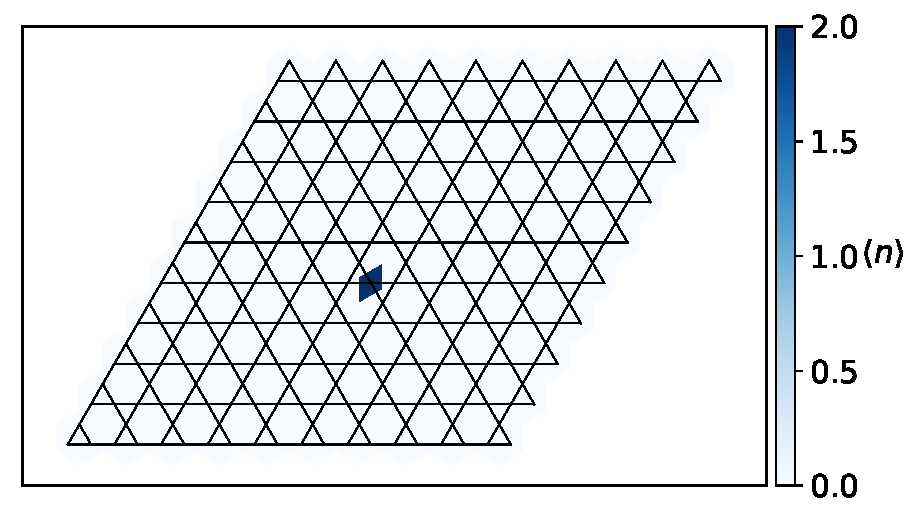
\includegraphics[width=0.45\textwidth]{Figures/Single_Site_Initial}\label{Fig:Single_Site_Initial}}\hfill
    \sidesubfloat[]{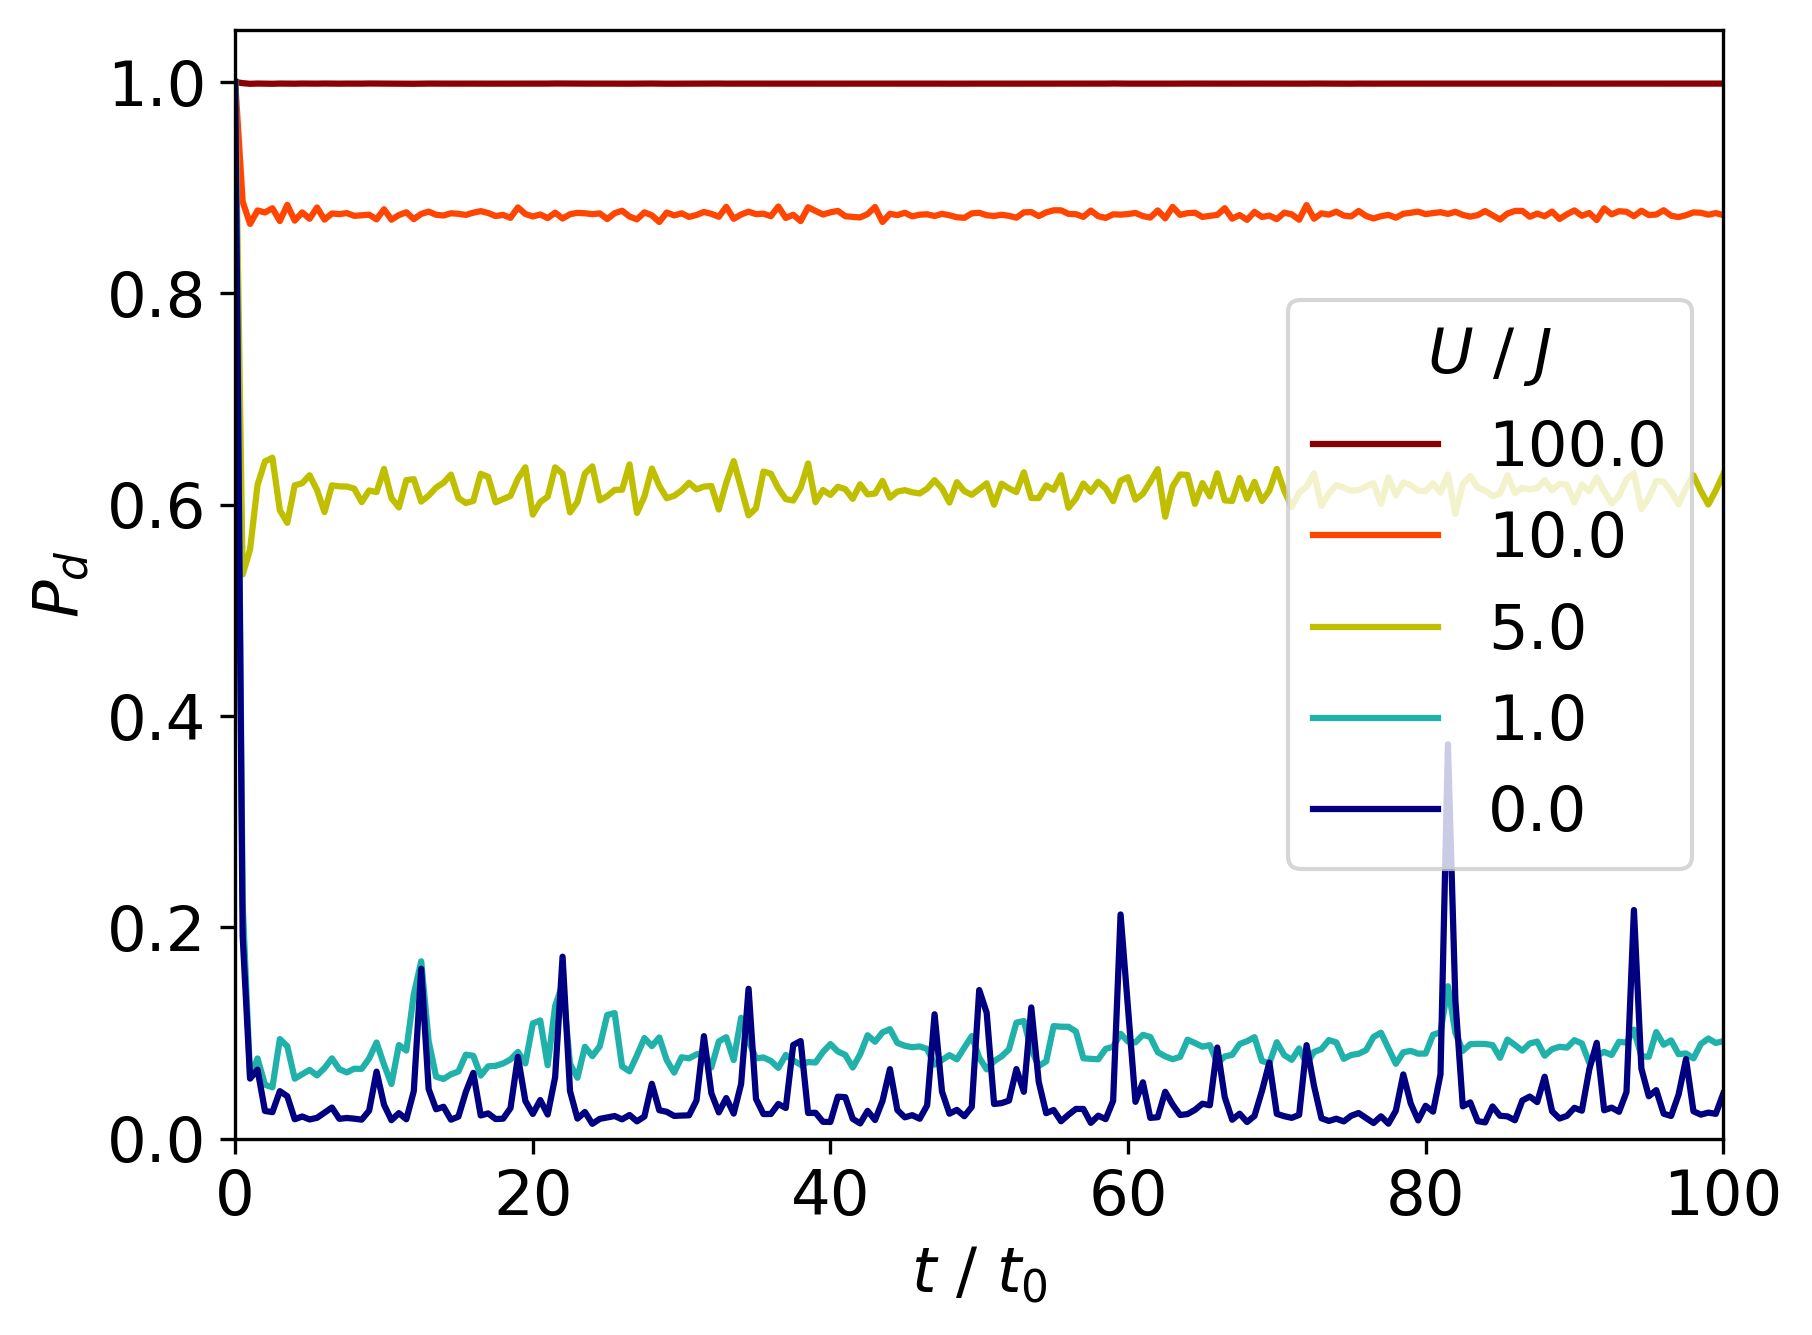
\includegraphics[height=5.6cm]{Figures/Pd_vs_t}\label{Fig:Pd_vs_t}}\hfill
    \sidesubfloat[]{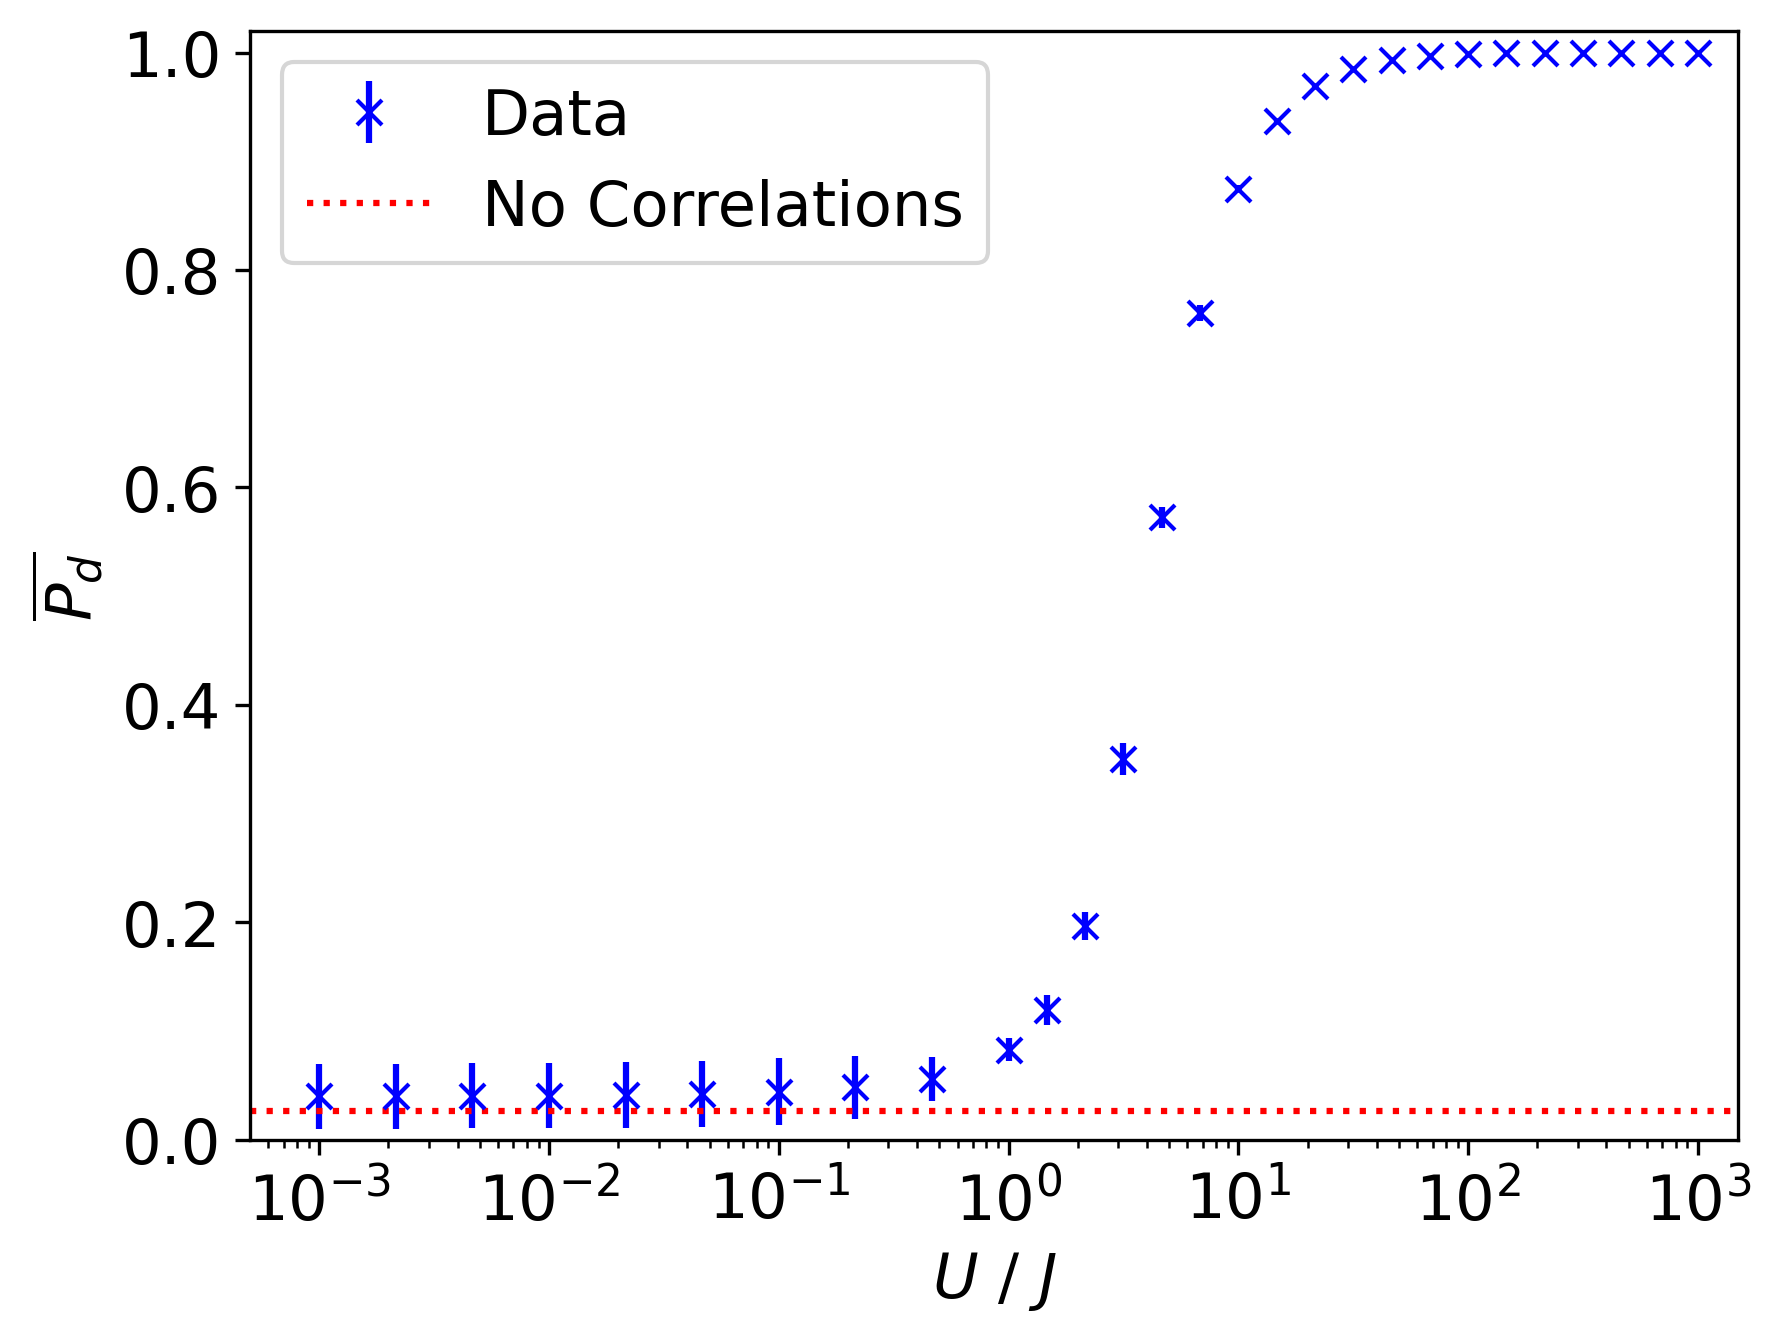
\includegraphics[height=5.6cm]{Figures/Pd_vs_U}\label{Fig:Pd_vs_U}}\hfill
    \sidesubfloat[]{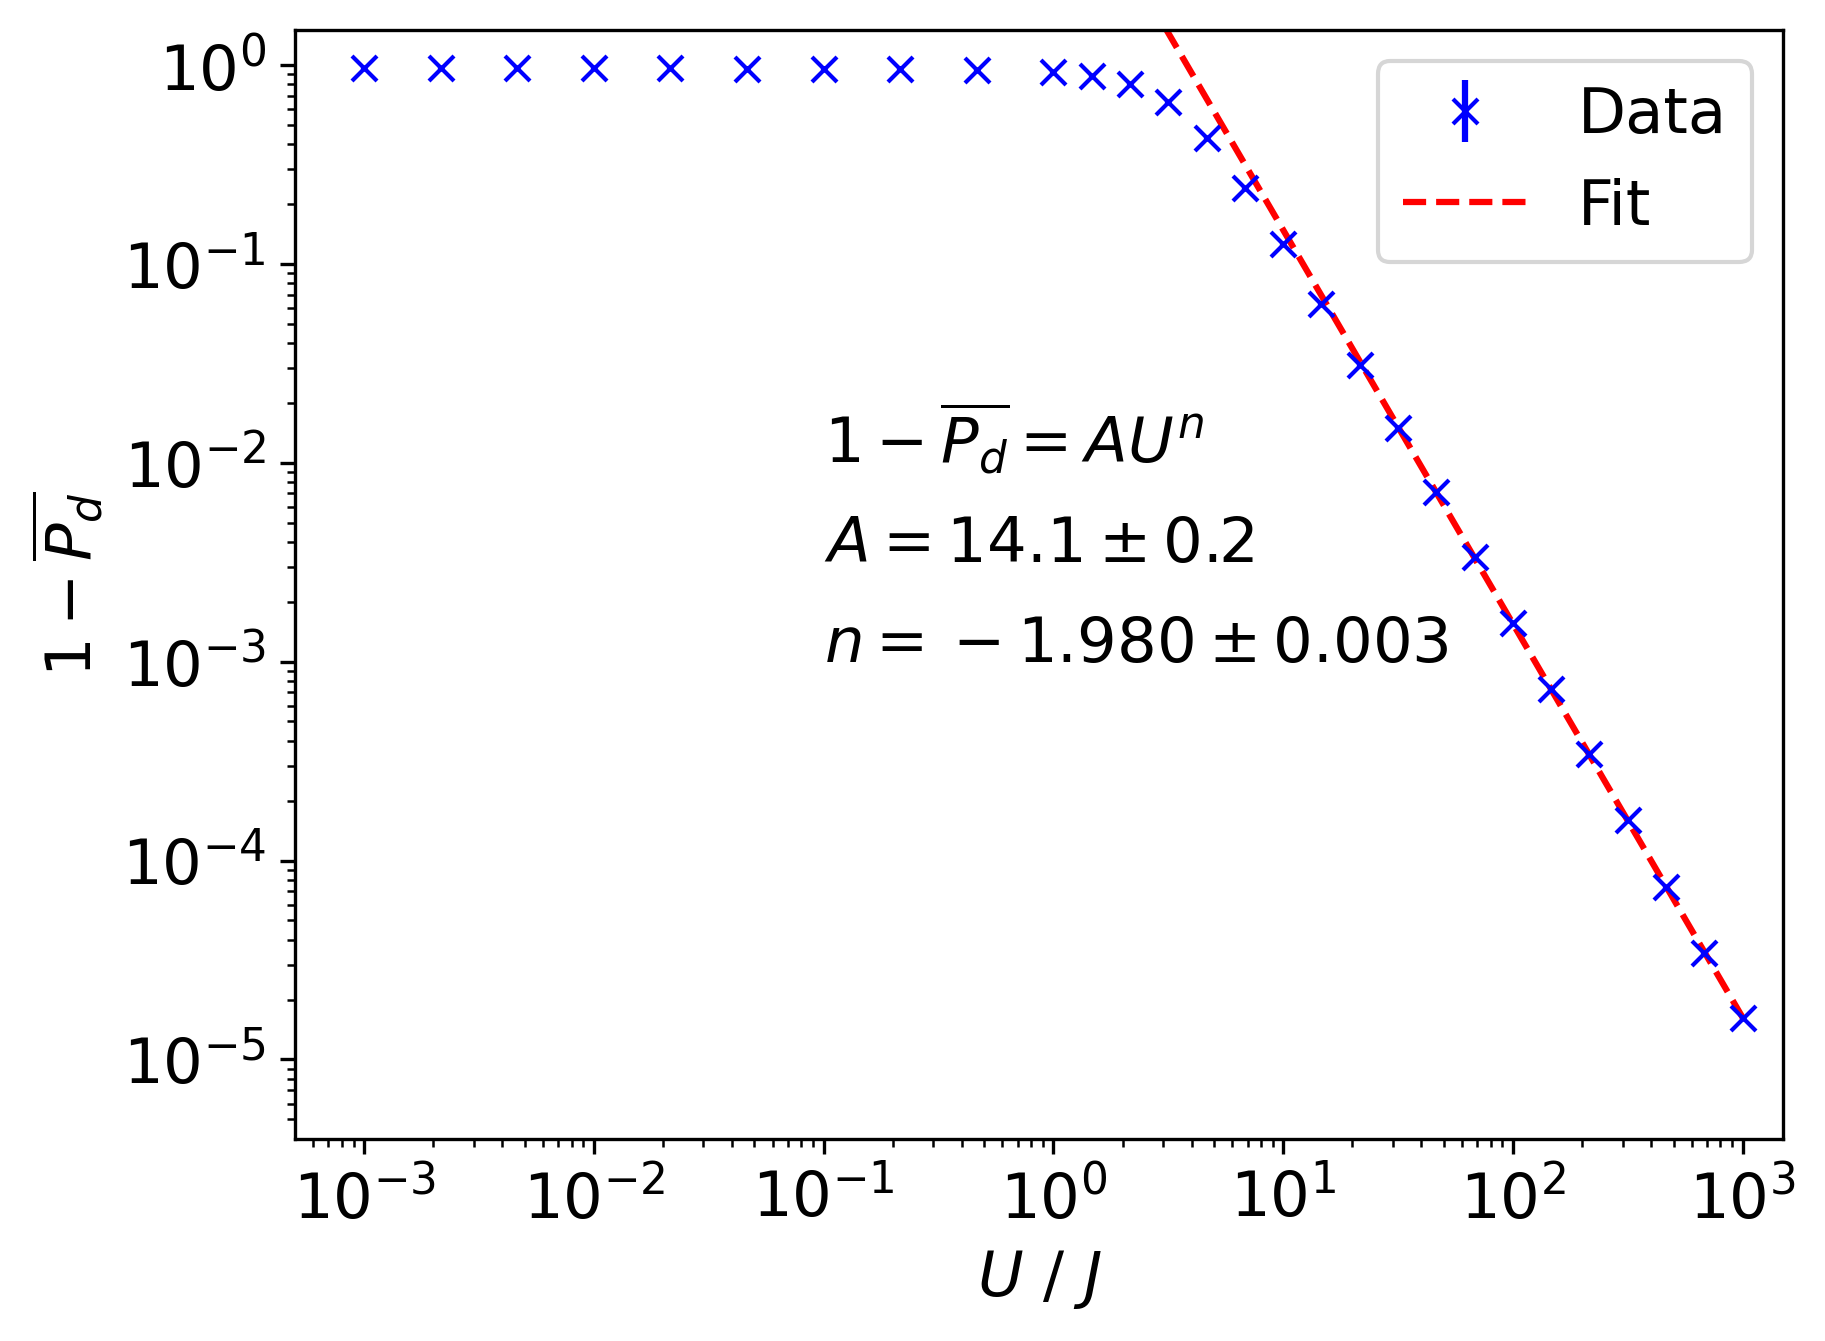
\includegraphics[height=5.6cm]{Figures/Pd_vs_U_log}\label{Fig:Pd_vs_U_log}}
    \caption{(a) Doublon probability against time for simulations with an initial doublon state, for various interaction strengths. (b) Doublon probability, averaged for $t\geq 10\, t_0$, against interaction strength. Error bars show standard deviations of the fluctuations. Red dotted line shows the value expected for no correlations, $N_{\text{sites}}/N_{\text{states}}$. (c) Time-averaged non-doublon probability against interaction strength, with log scale. The power law fit is performed to the data with $U\geq30$.}
    \label{Fig:Doublon_Probability}
\end{figure}